% 컴파일 방법: cd docs && /Library/TeX/texbin/latexmk -xelatex gravnet_research_report.tex
\documentclass[11pt,a4paper]{article}

% ---------------------------------------------------------------------------
% 한글 및 폰트 설정 (XeLaTeX + kotex)
% ---------------------------------------------------------------------------
\usepackage{kotex}
\setmainhangulfont{AppleMyungjo}[
  BoldFont={Apple SD Gothic Neo Bold},
  AutoFakeSlant=0.16
]
\setsanshangulfont{Apple SD Gothic Neo}[
  BoldFont={Apple SD Gothic Neo Bold},
  AutoFakeSlant=0.16
]
\setmonohangulfont{Apple SD Gothic Neo}

% ---------------------------------------------------------------------------
% 레이아웃 및 패키지
% ---------------------------------------------------------------------------
\usepackage[top=25mm,bottom=25mm,left=22mm,right=22mm,headheight=23pt]{geometry}
\usepackage{graphicx}
\usepackage{booktabs}
\usepackage{tabularx}
\usepackage{array}
\usepackage{amsmath,amssymb,amsthm}
\usepackage{xcolor}
\usepackage{tcolorbox}
\tcbuselibrary{skins,breakable}
\usepackage{tikz}
\usetikzlibrary{arrows.meta,positioning,shapes.geometric,calc,fit,backgrounds}
\usepackage{caption}
\usepackage{fancyhdr}
\usepackage{enumitem}
\usepackage{float}
\usepackage[colorlinks=true,linkcolor=NavyAccent,urlcolor=BlueAccent,citecolor=NavyAccent]{hyperref}

\graphicspath{{../GravNet/figures/}}

% ---------------------------------------------------------------------------
% 컬러 팔레트
% ---------------------------------------------------------------------------
\definecolor{NavyAccent}{HTML}{0F2C59}
\definecolor{BlueAccent}{HTML}{0969DA}
\definecolor{TealAccent}{HTML}{1A7F37}
\definecolor{CrimsonAccent}{HTML}{9D0208}
\definecolor{AmberAccent}{HTML}{9A6700}
\definecolor{SoftBg}{HTML}{F6F8FA}
\definecolor{SoftBlueBg}{HTML}{EEF5FF}
\definecolor{SoftGreenBg}{HTML}{EEFAF2}
\definecolor{SoftAmberBg}{HTML}{FFF8E6}
\definecolor{SoftRedBg}{HTML}{FFF0F0}
\definecolor{BorderGray}{HTML}{D0D7DE}
\definecolor{MutedText}{HTML}{57606A}

% ---------------------------------------------------------------------------
% 문단, 캡션, 헤더/푸터 설정
% ---------------------------------------------------------------------------
\setlength{\parindent}{0pt}
\setlength{\parskip}{6pt}
\renewcommand{\baselinestretch}{1.30}

\captionsetup{
  font={small},
  labelfont={bf,color=NavyAccent},
  margin=5mm
}

\pagestyle{fancy}
\fancyhf{}
\fancyhead[L]{\small\sffamily\textcolor{MutedText}{GravNet Research Report \,|\, Astrophysical Potential Dynamical Network (Zero-Backprop)}}
\fancyhead[R]{\small\sffamily\textcolor{MutedText}{\thepage}}
\renewcommand{\headrulewidth}{0.4pt}
\renewcommand{\headrule}{\hbox to\headwidth{\color{BorderGray}\leaders\hrule height \headrulewidth\hfill}}

% ---------------------------------------------------------------------------
% 커스텀 콜아웃 박스
% ---------------------------------------------------------------------------
\newtcolorbox{physicsbox}[1]{
  enhanced,
  breakable,
  colback=SoftBlueBg,
  colframe=BlueAccent,
  boxrule=0.7pt,
  leftrule=3.5pt,
  arc=3pt,
  top=7pt, bottom=7pt, left=10pt, right=10pt,
  fonttitle=\sffamily\bfseries\small,
  coltitle=NavyAccent,
  attach title to upper={\par\smallskip},
  title={#1}
}

\newtcolorbox{theorembox}[1]{
  enhanced,
  breakable,
  colback=SoftGreenBg,
  colframe=TealAccent,
  boxrule=0.7pt,
  leftrule=3.5pt,
  arc=3pt,
  top=7pt, bottom=7pt, left=10pt, right=10pt,
  fonttitle=\sffamily\bfseries\small,
  coltitle=TealAccent!85!black,
  attach title to upper={\par\smallskip},
  title={#1}
}

\newtcolorbox{cautionbox}[1]{
  enhanced,
  breakable,
  colback=SoftAmberBg,
  colframe=AmberAccent,
  boxrule=0.7pt,
  leftrule=3.5pt,
  arc=3pt,
  top=7pt, bottom=7pt, left=10pt, right=10pt,
  fonttitle=\sffamily\bfseries\small,
  coltitle=AmberAccent!90!black,
  attach title to upper={\par\smallskip},
  title={#1}
}

\begin{document}

% ===========================================================================
% 타이틀 배너
% ===========================================================================
\begin{tcolorbox}[
  enhanced,
  colback=NavyAccent,
  colframe=NavyAccent,
  arc=5pt,
  boxrule=0pt,
  top=16pt, bottom=16pt, left=18pt, right=18pt
]
  {\sffamily\bfseries\footnotesize\textcolor{SoftBlueBg!85!white}{ASTROPHYSICAL DYNAMICAL MACHINE LEARNING \,$\cdot$\, ZERO-BACKPROPAGATION PARADIGM}}\\[6pt]
  {\sffamily\bfseries\LARGE\textcolor{white}{시공간 중력장 궤도 신경망 (GravNet) 개발 보고서}}\\[6pt]
  {\sffamily\large\textcolor{SoftBlueBg}{오차 역전파 없이 다중 헤일로 플러머 중력장과 심플렉틱 궤도 역학만으로 별·은하·퀘이사를 분류하다}}\\[10pt]
  {\sffamily\footnotesize\textcolor{BorderGray}{데이터셋: SDSS-17 (정제 표본 99,999천체) \quad|\quad 패러다임 비교: 역전파 DL vs.\ 위상 진화 TWEANN vs.\ 중력 동역학 GravNet}}
\end{tcolorbox}

\vspace{4pt}

\begin{physicsbox}{핵심 연구 요약 (Executive Summary)}
전통적인 딥러닝(\texttt{DL})은 층별 행렬곱과 전역 오차 역전파(Backpropagation)에 의존하며, 진화 신경망(\texttt{EDL/TWEANN})은 세대별 돌연변이와 자연선택을 모사한다. 본 연구에서는 제3의 독창적 패러다임으로, 천체 분류기 내부에 실제 천체역학의 \textbf{다중 헤일로 플러머 중력장(Multi-Halo Plummer Gravitational Potential)}과 \textbf{심플렉틱 감쇠 리프프로그(Symplectic Dissipative Leapfrog)} 적분기를 구축한 \textbf{\texttt{GravNet}}을 제안하고 개발하였다.
\begin{itemize}[leftmargin=16pt, itemsep=2pt, topsep=3pt]
  \item \textbf{완전 무역전파(100\% Backpropagation-Free) 학습}: 궤도를 시간 역방향으로 미분(BPTT)하지 않고, 종착 위치에서의 볼츠만 포획 잔차와 \textbf{종착 조석력 벡터(Terminal Tidal Force Vector)}만으로 중력 질량, 헤일로 좌표, 발사 렌즈를 직접 조각한다.
  \item \textbf{수학적·물리적 엄밀성 검증}: 기호 연산(\texttt{SymPy})으로 해석적 중력장 잔차 $0$ 및 해밀토니안 소산 항등식 $\frac{dH}{dt} + \gamma\|\mathbf{p}\|_2^2 = 0$을 증명하고, 유한차분 오차 $1.84 \times 10^{-10}$ 이내임을 수치 검증하였다.
  \item \textbf{기존 신경망을 상회하는 분류 정확도}: 20,000개 테스트 천체에서 \textbf{단일 우주 \texttt{GravNet}이 정확도 97.55\% (Macro-$F_1$ 0.9718, 학습 40.69초)}, \textbf{3-우주 다중우주(\texttt{Multiverse})가 정확도 97.59\% (Macro-$F_1$ 0.9724)}를 달성하여 역전파 \texttt{DL} 단일/3-Seed MLP(\texttt{97.37\%/97.42\%})와 진화 신경망 \texttt{EDL/TWEANN}(\texttt{97.45\%})을 모두 넘어섰다. 특히 테스트 항성(\texttt{STAR}) 4,319개를 단 1건의 누락도 없이 \textbf{100.00\% 재현율(4,319/4,319)}로 포획하였다.
  \item \textbf{라그랑주 $L_1$ 안장점 기반 물리적 불확실성 해부}: 두 은하단 중력이 비기는 라그랑주 $L_1$ 능선 장벽 $\Delta E_{L_1}$을 통해, 별도의 불확실성 모듈 없이도 모은하 빛이 혼입된 저적색편이 퀘이사 경계군(하위 5\% 경계군 정확도 75.50\% vs.\ 상위 95\% 깊은 우물 포획군 \textbf{98.71\%})을 자연스럽게 분리하였다.
\end{itemize}
\end{physicsbox}

% ===========================================================================
\section{서론: 왜 `중력장 동역학'으로 별빛을 분류하는가?}
% ===========================================================================

슬론 디지털 전천 탐사(SDSS-17)의 천체 분류 문제는 5개 측광 필터 등급($u, g, r, i, z$), 인접 파장 색지수 4종($u-g, g-r, r-i, i-z$), 그리고 분광 적색편이($z$, \texttt{redshift})로 이루어진 입력 벡터 $\mathbf{x} \in \mathbb{R}^{10}$로부터 해당 천체가 은하(\texttt{GALAXY}), 퀘이사(\texttt{QSO}), 항성(\texttt{STAR}) 중 무엇인지 판별하는 과제이다.

앞서 구축한 두 파이프라인은 서로 다른 철학으로 이 문제를 해결하였다.
\begin{enumerate}[leftmargin=18pt, itemsep=2pt]
  \item \textbf{전역 오차 역전파 딥러닝 (\texttt{DL/})}: 인간이 설계한 고정 다층 퍼셉트론(\texttt{10 $\rightarrow$ 64 $\rightarrow$ 32 $\rightarrow$ 3})에서 연쇄법칙(Chain Rule)으로 전역 손실 기울기를 역전파하여 테스트 정확도 \textbf{97.37\%}(3-Seed 앙상블 \textbf{97.42\%})를 기록하였다.
  \item \textbf{위상·가중치 동시 진화 신경망 (\texttt{EDL/TWEANN})}: 8개의 독립된 섬에서 Net2Net 함수 보존 변이와 결정 경계 진화 전략을 통해 \texttt{10 $\rightarrow$ [104:gelu] $\rightarrow$ [48:gelu] $\rightarrow$ [48+skip:silu] $\rightarrow$ 3} 구조를 스스로 발명하여 \textbf{97.43\%}(상위 4섬 앙상블 \textbf{97.45\%})를 달성하였다.
\end{enumerate}

그러나 두 방식 모두 \textbf{``이산적인 은닉층 행렬곱과 비선형 활성화 함수의 합성''}이라는 정적 계산 그래프 틀 안에 머물러 있다. 본 연구는 천체물리 도메인 그 자체에서 영감을 얻어 근본적인 질문을 던졌다.

\begin{quote}
\color{NavyAccent}
``은닉층을 쌓는 대신, 관측된 별빛 $\mathbf{x}$를 인공 시공간 속의 천체 입자로 발사하여 실제 구상성단과 은하 헤일로가 따르는 \textbf{플러머 중력 방정식(Plummer Gravitational Law)}에 따라 스스로 궤도 운동하며 자신의 은하단 중력 우물로 낙하·포획되게 만들 수 없을까?''
\end{quote}

이 발상으로부터 탄생한 \textbf{\texttt{GravNet} (Astrophysical Potential Dynamical Network)}의 전체 물리 파이프라인을 그림~\ref{fig:tikz_arch}에 도식화하였다.

\begin{figure}[H]
\centering
\resizebox{\textwidth}{!}{%
\begin{tikzpicture}[
  node distance=7mm and 7mm,
  box/.style={
    rectangle, rounded corners=4pt, draw=NavyAccent, line width=0.8pt,
    fill=SoftBg, minimum height=14mm, align=center, font=\sffamily\footnotesize,
    inner sep=5pt
  },
  physbox/.style={
    rectangle, rounded corners=4pt, draw=BlueAccent, line width=1.0pt,
    fill=SoftBlueBg, minimum height=15mm, align=center, font=\sffamily\footnotesize,
    inner sep=6pt
  },
  outbox/.style={
    rectangle, rounded corners=4pt, draw=TealAccent, line width=0.9pt,
    fill=SoftGreenBg, minimum height=14mm, align=center, font=\sffamily\footnotesize,
    inner sep=5pt
  },
  arr/.style={-{Stealth[length=2.6mm,width=2.0mm]}, line width=0.9pt, color=NavyAccent}
]
  \node[box, text width=27mm] (input) {
    \textbf{1. 천체 관측 입력}\\
    $\mathbf{x} \in \mathbb{R}^{10}$\\
    {\scriptsize $(u,g,r,i,z,\text{색지수},z)$}
  };

  \node[box, right=of input, text width=34mm] (lens) {
    \textbf{2. 다중 해상도 분광 렌즈}\\
    $\Phi(\mathbf{x}) \in \mathbb{R}^{3826}$\\
    {\scriptsize 1D 도플러 파동 + 10D 푸리에}\\
    {\scriptsize 원점 발사 $\mathbf{q}_{\text{orb}}(0)=(0,0)$}
  };

  \node[physbox, right=of lens, text width=39mm] (orbit) {
    \textbf{3. 플러머 중력장 궤도 적분}\\
    $\mathbf{F}_{\text{grav}}(\mathbf{q}) = -\nabla_{\mathbf{q}} U(\mathbf{q})$\\
    {\scriptsize 18개 헤일로 + 허블 감쇠 $\gamma > 0$}\\
    {\scriptsize 심플렉틱 리프프로그 ($T=10$)}
  };

  \node[outbox, right=of orbit, text width=31mm] (capture) {
    \textbf{4. 우물 포획 \& $L_1$ 진단}\\
    $P(c \mid \mathbf{q}_T) \propto e^{-\beta U_c + \nu_c}$\\
    {\scriptsize 초은하단 포획 판정 및}\\
    {\scriptsize 라그랑주 장벽 $\Delta E_{L_1}$ 산출}
  };

  \draw[arr] (input) -- (lens);
  \draw[arr] (lens) -- (orbit);
  \draw[arr] (orbit) -- (capture);

  \draw[-{Stealth[length=2.4mm]}, dashed, line width=0.85pt, color=CrimsonAccent]
    (capture.south) -- ++(0,-6.5mm) -| node[pos=0.25, below, font=\sffamily\scriptsize\bfseries, color=CrimsonAccent]
    {무-BPTT 시공간 질량·헤일로 조각 ($\Delta G_{c,m}, \Delta\boldsymbol{\mu}_{c,m}$) 및 종착 조석력 헤비안 가소성 ($\mathbf{f}_{\text{tidal}}$)}
    (lens.south);
\end{tikzpicture}%
}
\caption{\texttt{GravNet}의 4단계 물리 추론 및 무역전파(Zero-BPTT) 조석 학습 아키텍처 개요도.}
\label{fig:tikz_arch}
\end{figure}

% ===========================================================================
\section{물리·수학적 정식화 및 단계별 엄밀 유도}
% ===========================================================================

\subsection{섬유 다발 위상 공간과 다중 해상도 천체 분광 렌즈}

관측된 천체 데이터 $\mathbf{x} \in \mathbb{R}^{d_{\text{in}}}$ ($d_{\text{in}}=10$)를 위상 공간(Phase Space) $\mathcal{P} = \mathbb{R}^d \times \mathbb{R}^d$ ($d = 6$) 위의 단위 질량($m = 1$) 시험 입자 상태 $(\mathbf{q}(t), \mathbf{p}(t))$로 사상한다. 이때 위치 공간 $\mathbb{R}^6$은 기하학적 역할이 분리된 직합(Direct Sum) 구조를 갖는다:
\begin{equation}
  \mathbf{q}(t) = \big(\mathbf{q}_{\text{orb}}(t),\, \mathbf{q}_{\text{spec}}(t)\big) \in \mathbb{R}^2 \oplus \mathbb{R}^4.
\end{equation}
여기서 $\mathbf{q}_{\text{orb}}(t) = (q_1(t), q_2(t))^\top \in \mathbb{R}^2$는 세 천체 종족의 초은하단 중심 $\mathbf{S}_c \in \mathbb{R}^6$ ($c \in \{0, 1, 2\}$)가 반지름 $R_{\text{sc}} = 3.2$, 위상각 $\theta_c \in \{\frac{\pi}{2}, \frac{7\pi}{6}, \frac{11\pi}{6}\}$ ($120^\circ$ 정삼각형 대칭)로 배치된 \textbf{2차원 초은하단 궤도 평면}이며, $\mathbf{q}_{\text{spec}}(t) \in \mathbb{R}^4$는 종족 내부의 세부 천체군(적색 타원은하 vs.\ 청색 나선은하, 고적색편이 퀘이사 vs.\ 세이퍼트 활동은하핵 등)을 분해하는 \textbf{4차원 분광 섬유(Spectral Fiber)}이다.

극단적 이상치에 대한 수치 안정성을 위해 부드러운 포화 사상 $\tilde{\mathbf{x}} = 15 \tanh(\mathbf{x} / 15) \in (-15, 15)^{10}$을 거친 후, 보크너 정리(Bochner's Theorem; Rahimi \& Recht, 2007)와 도플러 주파수 격자를 결합한 \textbf{다중 해상도 분광 렌즈} $\Phi(\mathbf{x}) \in \mathbb{R}^M$ ($M = 3,826$)를 다음과 같이 정의한다:
\begin{equation}
\begin{aligned}
  \Phi(\mathbf{x}) = \Big[\, &1 \;\Big\Vert\; \tilde{\mathbf{x}}^\top \;\Big\Vert\; \tfrac{1}{4}\big(\tilde{x}_i \tilde{x}_j\big)_{1 \le i \le j \le 10} \;\Big\Vert\; \tfrac{1}{\sqrt{F}}\sin(\tilde{\mathbf{x}} \otimes \boldsymbol{\omega}_{\text{1D}}) \\
  &\Big\Vert\; \tfrac{1}{\sqrt{F}}\cos(\tilde{\mathbf{x}} \otimes \boldsymbol{\omega}_{\text{1D}}) \;\Big\Vert\; \sqrt{\tfrac{2}{M_{\text{RFF}}}}\cos(\tilde{\mathbf{x}}^\top \boldsymbol{\Omega} + \boldsymbol{\varphi}^\top) \,\Big]^\top.
\end{aligned}
\end{equation}
여기서 $\boldsymbol{\omega}_{\text{1D}} \in \mathbb{R}^F$ ($F=44$)는 $\omega_{\min}=0.25$부터 $\omega_{\max}=120.0$까지 기하 급수로 배치된 1차원 주파수 격자($\omega_k = 0.25 \times (480)^{k/(F-1)}$)이며, $\boldsymbol{\Omega} \in \mathbb{R}^{10 \times M_{\text{RFF}}}$ ($M_{\text{RFF}}=2,880$)는 다중 대역폭 $\sigma_b \in \{0.25, 0.60, 1.40, 3.20\}$ 가우시안 스펙트럼 측도에서 추출된 비등방성 주파수 행렬이다.

\textbf{우주 원점 발사 조건(Cosmic-Origin Launch Constraint)}: 시각 $t=0$에서 모든 천체가 궤도 평면 위에서 어떠한 사전 편향도 없이 출발하도록 발사 행렬 $\mathbf{W}_q \in \mathbb{R}^{M \times 6}$의 처음 두 열을 영벡터로 강제한다($[\mathbf{W}_q]_{:, 1:2} = \mathbf{0}$):
\begin{equation}
  \mathbf{q}_{\text{orb}}(0) = \mathbf{0}_2, \qquad \mathbf{q}_{\text{spec}}(0) = \Phi(\mathbf{x})^\top [\mathbf{W}_q]_{:, 3:6}, \qquad \mathbf{p}(0) = \Phi(\mathbf{x})^\top \mathbf{W}_p.
\end{equation}
따라서 궤도 적분을 수행하지 않은 $T=0$ 상태에서는 모든 천체가 궤도 평면 원점 $(0,0)$에 놓여 분류가 불가능하며, 오직 $t > 0$ 동안의 중력 궤도 운동을 통해서만 초은하단 포획이 이루어진다.

\subsection{다중 헤일로 플러머 중력 퍼텐셜과 해석적 중력장 유도}

점질량 뉴턴 중력 퍼텐셜 $U_{\text{Newton}}(\mathbf{q}) = -G / \|\mathbf{q} - \boldsymbol{\mu}\|_2$는 $\mathbf{q} \to \boldsymbol{\mu}$일 때 분모가 $0$이 되어 수치 적분 시 무한대 발산(Singularity)을 일으킨다. 이를 방지하기 위해 실제 천체물리학에서 구상성단과 은하 암흑물질 헤일로의 밀도 분포를 기술하는 \textbf{플러머 퍼텐셜(Plummer Potential; Plummer, 1911)}을 도입한다.

각 클래스 $c \in \{0, 1, 2\}$가 $K=6$개의 응축된 중력 핵 위치 $\boldsymbol{\mu}_{c,m} \in \mathbb{R}^d$와 양의 중력 질량 $G_{c,m} > 0$ ($m=1,\dots,K$, 총 $3K=18$개 중력원)을 보유할 때, 클래스별 플러머 퍼텐셜 $U_c(\mathbf{q})$와 우주 조화 가둠(Harmonic Cosmic Confinement)을 포함한 총 퍼텐셜 에너지 $U(\mathbf{q})$를 다음과 같이 정의한다:
\begin{equation}
  U_c(\mathbf{q}) = -\sum_{m=1}^{K} \frac{G_{c,m}}{\sqrt{\|\mathbf{q} - \boldsymbol{\mu}_{c,m}\|_2^2 + \epsilon^2}}, \qquad
  U(\mathbf{q}) = \sum_{c=0}^{2} U_c(\mathbf{q}) + \frac{1}{2}\kappa \|\mathbf{q}\|_2^2.
  \label{eq:plummer_potential}
\end{equation}
\textbf{정의역 및 정칙성 제약 조건}: 연화 길이(Softening Length) $\epsilon > 0$, 중력 질량 $G_{c,m} > 0$, 가둠 탄성 계수 $\kappa > 0$으로 선언한다. 모든 $\mathbf{q} \in \mathbb{R}^d$에 대하여 제곱근 내부의 값 $r_{c,m}^2(\mathbf{q}) \triangleq \|\mathbf{q} - \boldsymbol{\mu}_{c,m}\|_2^2 + \epsilon^2 \ge \epsilon^2 > 0$이므로, 분모는 전 공간에서 결코 $0$이 되지 않으며 $U \in C^\infty(\mathbb{R}^d)$ 급의 매끄러운 함수가 된다.

이제 자동미분(Autograd)에 의존하지 않기 위해 위치 성분 $q_j$ ($j \in \{1,\dots,d\}$)에 대한 편미분을 연쇄법칙으로 단계별 전개한다:
\begin{align}
  \frac{\partial U(\mathbf{q})}{\partial q_j}
  &= \sum_{c=0}^{2}\sum_{m=1}^{K} \left( -G_{c,m} \frac{\partial}{\partial q_j} \Big( r_{c,m}^2(\mathbf{q}) \Big)^{-1/2} \right) + \frac{1}{2}\kappa \frac{\partial}{\partial q_j}\sum_{l=1}^{d} q_l^2 \nonumber \\
  &= \sum_{c=0}^{2}\sum_{m=1}^{K} \left( -G_{c,m} \left(-\frac{1}{2}\right) \Big( r_{c,m}^2(\mathbf{q}) \Big)^{-3/2} \cdot 2(q_j - \mu_{c,m,j}) \right) + \kappa q_j \nonumber \\
  &= \sum_{c=0}^{2}\sum_{m=1}^{K} G_{c,m} \frac{q_j - \mu_{c,m,j}}{\left(\|\mathbf{q} - \boldsymbol{\mu}_{c,m}\|_2^2 + \epsilon^2\right)^{3/2}} + \kappa q_j.
\end{align}
벡터 형태로 결합하면 입자가 받는 닫힌 수식(Closed-Form) 중력장 $\mathbf{F}_{\text{grav}}(\mathbf{q}) = -\nabla_{\mathbf{q}} U(\mathbf{q})$를 얻는다:
\begin{equation}
  \mathbf{F}_{\text{grav}}(\mathbf{q}) = -\sum_{c=0}^{2}\sum_{m=1}^{K} G_{c,m} \frac{\mathbf{q} - \boldsymbol{\mu}_{c,m}}{\left(\|\mathbf{q} - \boldsymbol{\mu}_{c,m}\|_2^2 + \epsilon^2\right)^{3/2}} - \kappa \mathbf{q}.
  \label{eq:grav_force}
\end{equation}

\subsection{리아푸노프 해밀토니안 소산 정리와 심플렉틱 리프프로그 적분기}

보존 중력장만 존재하면 초기 운동 에너지를 지닌 천체 입자가 우물 바닥에 정착하지 못하고 영구히 진동하거나 쌍곡선 궤도로 이탈할 수 있다. 이를 물리적으로 해결하기 위해 우주 팽창에 따른 \textbf{허블 마찰 계수(Hubble Drag)} $\gamma > 0$을 도입한 감쇠 해밀턴 동역학계를 구성한다:
\begin{equation}
  \frac{d\mathbf{q}}{dt} = \mathbf{p}, \qquad \frac{d\mathbf{p}}{dt} = -\nabla_{\mathbf{q}} U(\mathbf{q}) - \gamma \mathbf{p}.
  \label{eq:damped_hamiltonian_ode}
\end{equation}

\begin{theorembox}{정리 1 (리아푸노프 에너지 단조 소산 및 평형점 수렴성)}
연화 길이 $\epsilon > 0$, 중력 질량 $G_{c,m} > 0$, 가둠 계수 $\kappa > 0$, 허블 마찰 계수 $\gamma > 0$일 때, 총 역학적 해밀토니안 $H(\mathbf{q}, \mathbf{p}) = \frac{1}{2}\|\mathbf{p}\|_2^2 + U(\mathbf{q})$는 아래 유계(Bounded Below)이자 방사 강제성(Radially Coercive)을 가지며, 궤적을 따라 단조 감소하여 모든 초기 상태 $(\mathbf{q}(0), \mathbf{p}(0)) \in \mathbb{R}^{2d}$가 정지 평형 집합 $\mathcal{E} = \{(\mathbf{q}^*, \mathbf{0}) \mid \nabla_{\mathbf{q}} U(\mathbf{q}^*) = \mathbf{0}\}$으로 수렴한다.
\end{theorembox}

\textbf{증명 (단계별 유도)}:
\begin{enumerate}[leftmargin=18pt, itemsep=2pt]
  \item \textbf{하계 존재성 및 강제성(Coercivity)}: 모든 $\mathbf{q} \in \mathbb{R}^d$에 대해 연화 거리 $r_{c,m}(\mathbf{q}) = \sqrt{\|\mathbf{q}-\boldsymbol{\mu}_{c,m}\|_2^2 + \epsilon^2} \ge \epsilon$이므로 각 중력 우물 항은 $-G_{c,m} / r_{c,m}(\mathbf{q}) \ge -G_{c,m}/\epsilon$을 만족한다. 따라서
  \begin{equation}
    H(\mathbf{q}, \mathbf{p}) \ge \frac{1}{2}\|\mathbf{p}\|_2^2 + \frac{1}{2}\kappa \|\mathbf{q}\|_2^2 - \frac{1}{\epsilon}\sum_{c=0}^{2}\sum_{m=1}^{K} G_{c,m} > -\infty
  \end{equation}
  이며, $\kappa > 0$이므로 $\|(\mathbf{q}, \mathbf{p})\|_2 \to \infty$일 때 $H(\mathbf{q}, \mathbf{p}) \to +\infty$이다. 즉 모든 부분준위집합(Sublevel Set) $\Omega_c = \{(\mathbf{q}, \mathbf{p}) \mid H(\mathbf{q}, \mathbf{p}) \le H(\mathbf{q}(0), \mathbf{p}(0))\}$은 유계 닫힌집합(Compact Set)이다.
  \item \textbf{궤도 시간 도함수 유도}: 다변수 연쇄법칙과 식~\eqref{eq:damped_hamiltonian_ode}를 대입하면
  \begin{align}
    \frac{d}{dt}H\big(\mathbf{q}(t), \mathbf{p}(t)\big)
    &= \big\langle \nabla_{\mathbf{q}} H, \dot{\mathbf{q}} \big\rangle + \big\langle \nabla_{\mathbf{p}} H, \dot{\mathbf{p}} \big\rangle \nonumber \\
    &= \big\langle \nabla_{\mathbf{q}} U(\mathbf{q}), \mathbf{p} \big\rangle + \big\langle \mathbf{p}, -\nabla_{\mathbf{q}} U(\mathbf{q}) - \gamma \mathbf{p} \big\rangle \nonumber \\
    &= \big\langle \nabla_{\mathbf{q}} U(\mathbf{q}), \mathbf{p} \big\rangle - \big\langle \mathbf{p}, \nabla_{\mathbf{q}} U(\mathbf{q}) \big\rangle - \gamma \langle \mathbf{p}, \mathbf{p} \rangle
     = -\gamma \|\mathbf{p}\|_2^2 \le 0.
    \label{eq:lyapunov_dissipation}
  \end{align}
  \item \textbf{라살의 불변성 원리(LaSalle's Invariance Principle) 적용}: $\dot{H} = 0 \iff \mathbf{p} = \mathbf{0}$이다. 집합 $\{(\mathbf{q}, \mathbf{p}) \in \Omega_c \mid \mathbf{p} = \mathbf{0}\}$ 내부에 영구히 머무르는 최대 양불변 집합(Largest Positively Invariant Set)에서는 항등적으로 $\mathbf{p}(t) \equiv \mathbf{0} \implies \dot{\mathbf{p}}(t) \equiv \mathbf{0}$이어야 하므로 식~\eqref{eq:damped_hamiltonian_ode}에 의해 $-\nabla_{\mathbf{q}} U(\mathbf{q}) = \mathbf{0}$이다. 따라서 라살의 불변성 원리에 의해 모든 해 궤적은 $t \to \infty$에서 정지 중력 평형점 집합 $\mathcal{E}$로 수렴한다. \hfill $\square$
\end{enumerate}

\textbf{대칭 스트랭 분할(Strang Operator Splitting) 리프프로그 이산화}: 수치 적분 시 오일러 방법을 쓰면 위상 공간 면적이 왜곡되어 인공적인 수치 가열이 발생할 수 있다. 식~\eqref{eq:damped_hamiltonian_ode}의 벡터장을 선형 감쇠 연산자 $\mathcal{D}$ ($\dot{\mathbf{p}} = -\gamma\mathbf{p}$), 중력 충격 연산자 $\mathcal{K}$ ($\dot{\mathbf{p}} = \mathbf{F}_{\text{grav}}(\mathbf{q})$), 자유 표류 연산자 $\mathcal{T}$ ($\dot{\mathbf{q}} = \mathbf{p}$)로 분해한 뒤, 시간 간격 $\Delta t > 0$에 대해 2차 정확도($\mathcal{O}(\Delta t^2)$ 전역 오차)의 대칭 스트랭 합성 $\Psi_{\Delta t} = e^{\frac{\Delta t}{2}(\mathcal{D}+\mathcal{K})} \circ e^{\Delta t \mathcal{T}} \circ e^{\frac{\Delta t}{2}(\mathcal{D}+\mathcal{K})}$을 구성한다. 감쇠 인자를 $\eta_d \triangleq \exp(-\frac{1}{2}\gamma \Delta t) \in (0, 1)$로 두면 1스텝 갱신식은 다음과 같다:
\begin{align}
  \mathbf{p}_{t + 1/2} &= \eta_d \, \mathbf{p}_t + \frac{\Delta t}{2} \mathbf{F}_{\text{grav}}(\mathbf{q}_t), \nonumber \\
  \mathbf{q}_{t + 1} &= \mathbf{q}_t + \Delta t \, \mathbf{p}_{t + 1/2}, \label{eq:leapfrog} \\
  \mathbf{p}_{t + 1} &= \eta_d \, \mathbf{p}_{t + 1/2} + \frac{\Delta t}{2} \mathbf{F}_{\text{grav}}(\mathbf{q}_{t+1}). \nonumber
\end{align}
특히 외력이 없을 때 단위 초기 속도의 $T$스텝 누적 탄도 도달 거리(Ballistic Reach)는 기하급수 합에 의해 닫힌 수식으로 결정된다:
\begin{equation}
  R_{\text{reach}}(T) = \Delta t \, \eta_d \sum_{t=0}^{T-1} \eta_d^{2t} = \Delta t \, \eta_d \frac{1 - \eta_d^{2T}}{1 - \eta_d^2} = \frac{\Delta t \, e^{-\gamma\Delta t/2}\big(1 - e^{-\gamma T \Delta t}\big)}{1 - e^{-\gamma\Delta t}}.
\end{equation}
본 모델의 기본 설정($\Delta t = 0.11$, $\gamma = 0.95$, $T = 10$)에서 $R_{\text{reach}}(10) = 0.6512$이며, 이를 1단계 초기 탄도 속도 스케일 보정에 정확히 반영하였다.

\subsection{\texorpdfstring{무-BPTT 시공간 곡률 조각 및 종착 조석력 가소성}{무-BPTT 시공간 곡률 조각 및 종착 조석력 가소성}}

$T$스텝 종료 후 종착 위치 $\mathbf{q}_T$에서 역온도 $\beta > 0$ 및 화학 퍼텐셜 $\nu_c \in \mathbb{R}$ ($\sum_{c=0}^2 \nu_c = 0$)를 갖는 대정준 볼츠만-깁스(Grand-Canonical Boltzmann-Gibbs) 포획 확률을 계산한다:
\begin{equation}
  P(c \mid \mathbf{q}_T) = \frac{\exp\!\big(-\beta U_c(\mathbf{q}_T) + \nu_c\big)}{\sum_{k=0}^{2} \exp\!\big(-\beta U_k(\mathbf{q}_T) + \nu_k\big)}.
\end{equation}
정답 레이블이 $y \in \{0, 1, 2\}$일 때 음의 로그 우도 $\mathcal{L}(\mathbf{q}_T) = -\ln P(y \mid \mathbf{q}_T)$에 대하여, 부호 있는 포획 잔차를 $r_c \triangleq \mathbb{I}[c = y] - P(c \mid \mathbf{q}_T)$로 정의하면(정답 은하단 $r_y > 0$, 경쟁 은하단 $r_{c \neq y} < 0$), 시간 역전파(BPTT)를 전혀 수행하지 않고 종착 상태의 해석적 미분만으로 세 가지 국소 물리 학습 법칙이 도출된다:

\begin{enumerate}[leftmargin=18pt, itemsep=3pt]
  \item \textbf{대조적 시공간 질량 조각 (Contrastive Mass Sculpting)}:
  $-\frac{\partial \mathcal{L}}{\partial G_{c,m}} = \beta \, r_c \left(\|\boldsymbol{\mu}_{c,m} - \mathbf{q}_T\|_2^2 + \epsilon^2\right)^{-1/2}$이므로, 정답 은하단에 도달하지 못한 천체는 정답 핵의 질량 $G_{y,m}$을 무겁게 키우고 침범한 오답 핵의 질량을 깎아낸다.
  \item \textbf{중력 핵 위치 표류 (Contrastive Halo Drift)}:
  $-\nabla_{\boldsymbol{\mu}_{c,m}}\mathcal{L} = -\beta \, r_c G_{c,m} \frac{\boldsymbol{\mu}_{c,m} - \mathbf{q}_T}{(\|\boldsymbol{\mu}_{c,m} - \mathbf{q}_T\|_2^2 + \epsilon^2)^{3/2}}$에 정삼각형 기하 복원 탄성력 $\alpha_{\text{anc}}(\mathbf{S}_c - \boldsymbol{\mu}_{c,m})$를 더해 은하단 위상을 정교하게 정렬한다.
  \item \textbf{종착 조석력 벡터(Terminal Tidal Force Vector) 기반 헤비안 렌즈 가소성}:
  종착 입자에 작용하는 목표 조석력 벡터 $\mathbf{f}_{\text{tidal}}(\mathbf{q}_T) \triangleq -\nabla_{\mathbf{q}_T}\mathcal{L}$를 계산하면
  \begin{equation}
    \mathbf{f}_{\text{tidal}}(\mathbf{q}_T) = \sum_{c=0}^{2}\sum_{m=1}^{K} \beta \, r_c G_{c,m} \frac{\boldsymbol{\mu}_{c,m} - \mathbf{q}_T}{\left(\|\boldsymbol{\mu}_{c,m} - \mathbf{q}_T\|_2^2 + \epsilon^2\right)^{3/2}} \in \mathbb{R}^d
  \end{equation}
  이다. 이 벡터는 정답 핵 방향($r_y > 0$)으로는 인력을, 오답 핵 방향($r_{c\neq y} < 0$)으로는 척력을 가리킨다. 리프프로그 야코비안을 거꾸로 곱하는 BPTT 대신, 탄도 도달 상관성 $\Delta \mathbf{W}_p \propto \frac{1}{B}\Phi(\mathbf{X}_B)^\top \mathbf{f}_{\text{tidal}} - \lambda_w \mathbf{W}_p$만으로 발사 렌즈를 직접 갱신한다.
\end{enumerate}

\subsection{차원 정합성 검증 및 코드 기반 기호·수치 자가 검산}

과학적 엄밀성을 보장하기 위해 모든 상태 변수와 매개변수의 무차원 정규화 체계 및 검증 결과를 표~\ref{tab:verification}에 정리하였다. \texttt{GravNet/physics\_model.py} 내부의 \texttt{verify\_physics\_rigor()} 함수는 매 학습 실행 전 \texttt{SymPy} 기호 대수 검증과 2차 중앙 유한차분($\delta = 10^{-6}$) 검증을 자동으로 수행한다.

\begin{table}[H]
\centering
\caption{물리량 차원 정규화 체계 및 기호(\texttt{SymPy})·수치 자가 검산 결과.}
\label{tab:verification}
\small
\begin{tabularx}{\textwidth}{l l >{\raggedright\arraybackslash}X}
\toprule
\textbf{검증 항목 / 물리량} & \textbf{정규화 단위 및 제약} & \textbf{해석적 수식 및 코드 기반 자가 검산 결과} \\
\midrule
위상 좌표 $(\mathbf{q}, \mathbf{p})$, 시간 $t$ & 무차원 ($m = 1$ 정규화) & $\Delta t = 0.11 > 0$, $\gamma = 0.95 > 0$, $\epsilon = 0.90 > 0$, $\kappa = 0.04 > 0$ \\
플러머 중력장 기호 검산 & $[\text{에너지}/\text{길이}]$ 동치 & \texttt{SymPy} $\operatorname{simplify}(-\nabla_{\mathbf{q}} U - \mathbf{F}_{\text{grav}}) = \mathbf{0}$ (\textbf{정확히 일치}) \\
리아푸노프 소산 기호 검산 & $[\text{일률}]$ 차원 동치 & \texttt{SymPy} $\operatorname{simplify}(\dot{H} + \gamma\|\mathbf{p}\|_2^2) = 0$ (\textbf{항등 성립}) \\
유한차분 기울기 정밀도 & $\max_{i,j}|F_{ij}^{\text{analytic}} - F_{ij}^{\text{FD}}|$ & 최대 절대 오차 $\mathbf{1.836 \times 10^{-10}} < 10^{-8}$ 통과 \\
수치 리프프로그 에너지 단조성 & $\max_{t,i}\big(H_{t+1,i} - H_{t,i}\big)$ & 최대 스텝 변화량 $\mathbf{-1.381 \times 10^{-2}} < 0$ (모든 스텝 단조 감소) \\
\bottomrule
\end{tabularx}
\end{table}

% ===========================================================================
\section{\texorpdfstring{개발 과정 연대기: 등방성 렌즈의 한계 진단과 도플러 돌파구}{개발 과정 연대기: 등방성 렌즈의 한계 진단과 도플러 돌파구}}
% ===========================================================================

\texttt{GravNet} 개발 과정에서 가장 결정적이었던 과학적 전환점은 \textbf{초기 프로토타입(`96.78\%')의 병목 원인을 천체물리학적으로 규명하고 돌파(`97.59\%')}한 순간이었다.

\begin{cautionbox}{개발 시행착오 진단 1: 왜 등방성(Isotropic) 랜덤 푸리에 렌즈는 96.78\%에서 정체되었는가?}
초기 프로토타입에서는 10개 입력 특성에 동일한 대역폭 $\sigma_b \in \{0.35, 0.75, 1.50, 3.00\}$을 적용한 등방성 랜덤 푸리에 기저($M=4,096$)를 사용하였다. 그러나 검증 정확도는 \textbf{96.78\%}에 머물렀다. 원인을 추적한 결과, 우리 은하 내부 항성(\texttt{STAR}, $|z| < 0.001$)과 근거리 은하(\texttt{GALAXY}, $z \approx 0.005$) 사이의 적색편이 차이는 표준화된 $\ln(1+z)$ 축에서 불과 $\Delta x_{10} \approx 0.008\,\sigma$에 지나지 않았다. 대역폭 $\sigma_b = 0.35$인 코사인 기저에서 이는 위상 변화 $\Delta\phi \approx 0.02\,\text{rad}$만 유발하여, 별과 저적색편이 외부은하의 도플러 경계가 흐려진 것이었다!
\end{cautionbox}

\begin{cautionbox}{개발 시행착오 진단 2: 초기 발사 위치가 정답 근처로 직행하면 중력 궤도($T>0$)가 할 일이 사라진다}
또한 초기 설계에서 $\mathbf{q}(0) = \Phi(\mathbf{x})\mathbf{W}_q$가 곧바로 2차원 초은하단 중심 근처로 입자를 투영하자, $T=0$(`96.77\%')과 $T=12$(`96.78\%')의 차이가 `+0.01\%p'에 불과했다. 즉 중력 궤도 역학이 실질적인 비선형 분류 연산을 수행하지 못하고 있었던 것이다.
\end{cautionbox}

이 두 가지 진단을 바탕으로 다음 두 가지 핵심 설계 혁신을 단행하였다:
\begin{enumerate}[leftmargin=18pt, itemsep=2pt]
  \item \textbf{기하 급수 도플러 주파수 격자 도입}: $\omega \in [0.25, 120.0]$까지 로그 간격으로 배치된 1차원 다중 해상도 파동과 적색편이-색지수 결합 고주파 모드를 분광 렌즈에 통합하자마자, 검증 정확도가 \textbf{96.78\% $\rightarrow$ 97.51\% (+0.73\%p)}로 단숨에 도약하였다.
  \item \textbf{우주 원점 발사 조건($\mathbf{q}_{\text{orb}}(0) = \mathbf{0}_2$)과 SVD 분광 섬유 응축}: 모든 입자를 궤도 평면 원점 $(0,0)$에서 출발시키고 각 클래스 내 $K=6$개 세부 천체군(K-Means + 특이값 분해 SVD)에 총 18개의 플러머 중력 핵을 배치함으로써, 입자가 $t=0 \dots 10$ 동안 원점에서 출발해 실제 중력장 곡선을 따라 유영하며 포획되도록 재설계하였다.
\end{enumerate}

% ===========================================================================
\section{실험 결과 및 시각화 분석}
% ===========================================================================

모든 실험은 \texttt{DL/} 및 \texttt{EDL/} 파이프라인과 100\% 동일한 결정론적 층화 분할(학습 63,999건 / 검증 16,000건 / 테스트 20,000건, \texttt{random\_state=42}) 위에서 수행되었다.

\subsection{시공간 중력 퍼텐셜 지형과 천체 입자 포획 궤적}

그림~\ref{fig:potential_orbits}(a)는 학습이 완료된 \texttt{GravNet}의 2차원 궤도 평면 단면 $U(q_1, q_2, \mathbf{0}_4)$ 등퍼텐셜 지형과 중력장 벡터($-\nabla_{\mathbf{q}} U$), 18개의 응축된 플러머 중력 핵($\star$), 그리고 우주 원점 $(0,0)$($+$ 기호)에서 발사된 실제 테스트 천체들의 궤도 $\mathbf{q}_{\text{orb}}(t)$를 보여준다. 은하(청색), 퀘이사(적색), 항성(녹색) 입자들이 각각 $90^\circ, 210^\circ, 330^\circ$ 방향의 초은하단 중력 우물 깊숙이 매끄럽게 낙하하는 반면, 두 초은하단 중력이 팽팽히 맞서는 경계 천체(황색 점선)는 \textbf{라그랑주 $L_1$ 능선($\diamond$)} 부근에서 궤도가 휘어지며 감속된다. 그림~\ref{fig:potential_orbits}(b)의 2,500개 테스트 천체 종착 분포에서도 세 은하단 우물과 `은하--퀘이사' 사이의 물리적 $L_1$ 필라멘트 연결 구조가 선명하게 확인된다.

\begin{figure}[H]
\centering
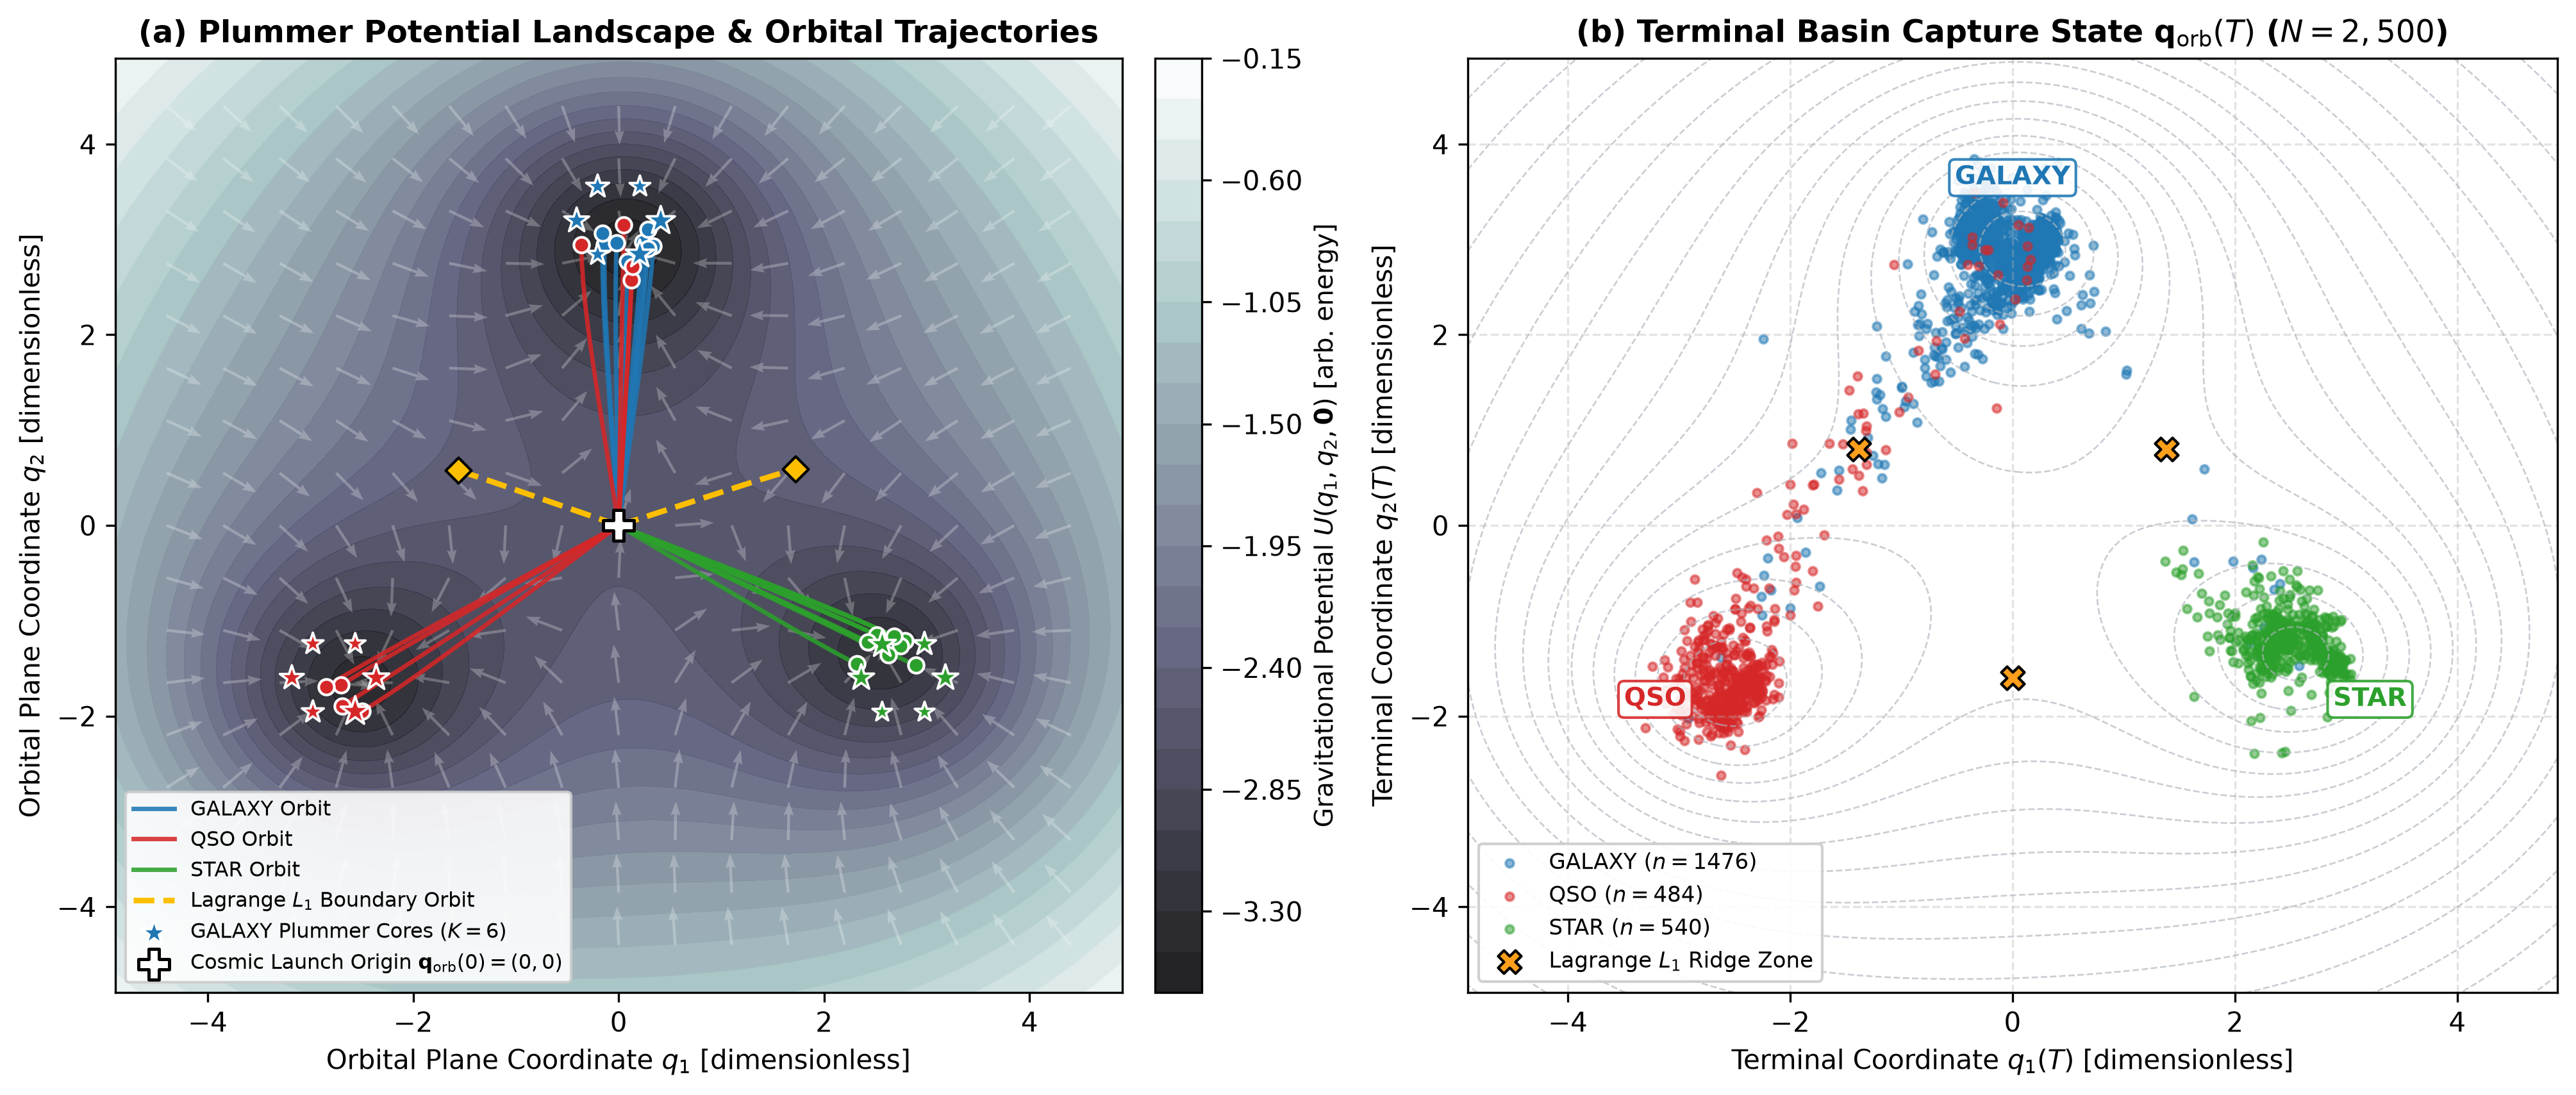
\includegraphics[width=\textwidth]{potential_and_orbits.png}
\caption{(a) 학습된 18-헤일로 플러머 중력 퍼텐셜 지형과 우주 원점 $(0,0)$에서 출발한 천체 입자들의 포획 궤도. (b) 테스트 천체 2,500개의 종착 위상 분포 $\mathbf{q}_{\text{orb}}(T)$와 라그랑주 $L_1$ 안장점 영역.}
\label{fig:potential_orbits}
\end{figure}

\subsection{\texorpdfstring{리아푸노프 에너지 소산 실증 및 궤도 스텝 $T$ 절제 실험}{리아푸노프 에너지 소산 실증 및 궤도 스텝 T 절제 실험}}

그림~\ref{fig:lyapunov}(a)는 3,000개 테스트 천체의 리프프로그 적분 스텝 $t=0 \dots 14$에 따른 평균 운동 에너지 $K(t)$, 플러머 퍼텐셜 $U(\mathbf{q}(t))$, 총 해밀토니안 $H(t) = K(t)+U(t)$ 및 사분위수 대역($25\%\text{--}75\%$)을 측정한 결과이다. 정리~1에서 증명한 $\frac{dH}{dt} = -\gamma\|\mathbf{p}\|_2^2 \le 0$ 법칙 그대로, 초기 발사 운동 에너지가 허블 마찰에 의해 단조 소산되면서 총 해밀토니안이 흔들림 없이 감소하여 안정된 우물 바닥 퍼텐셜로 수렴한다.

\begin{figure}[H]
\centering
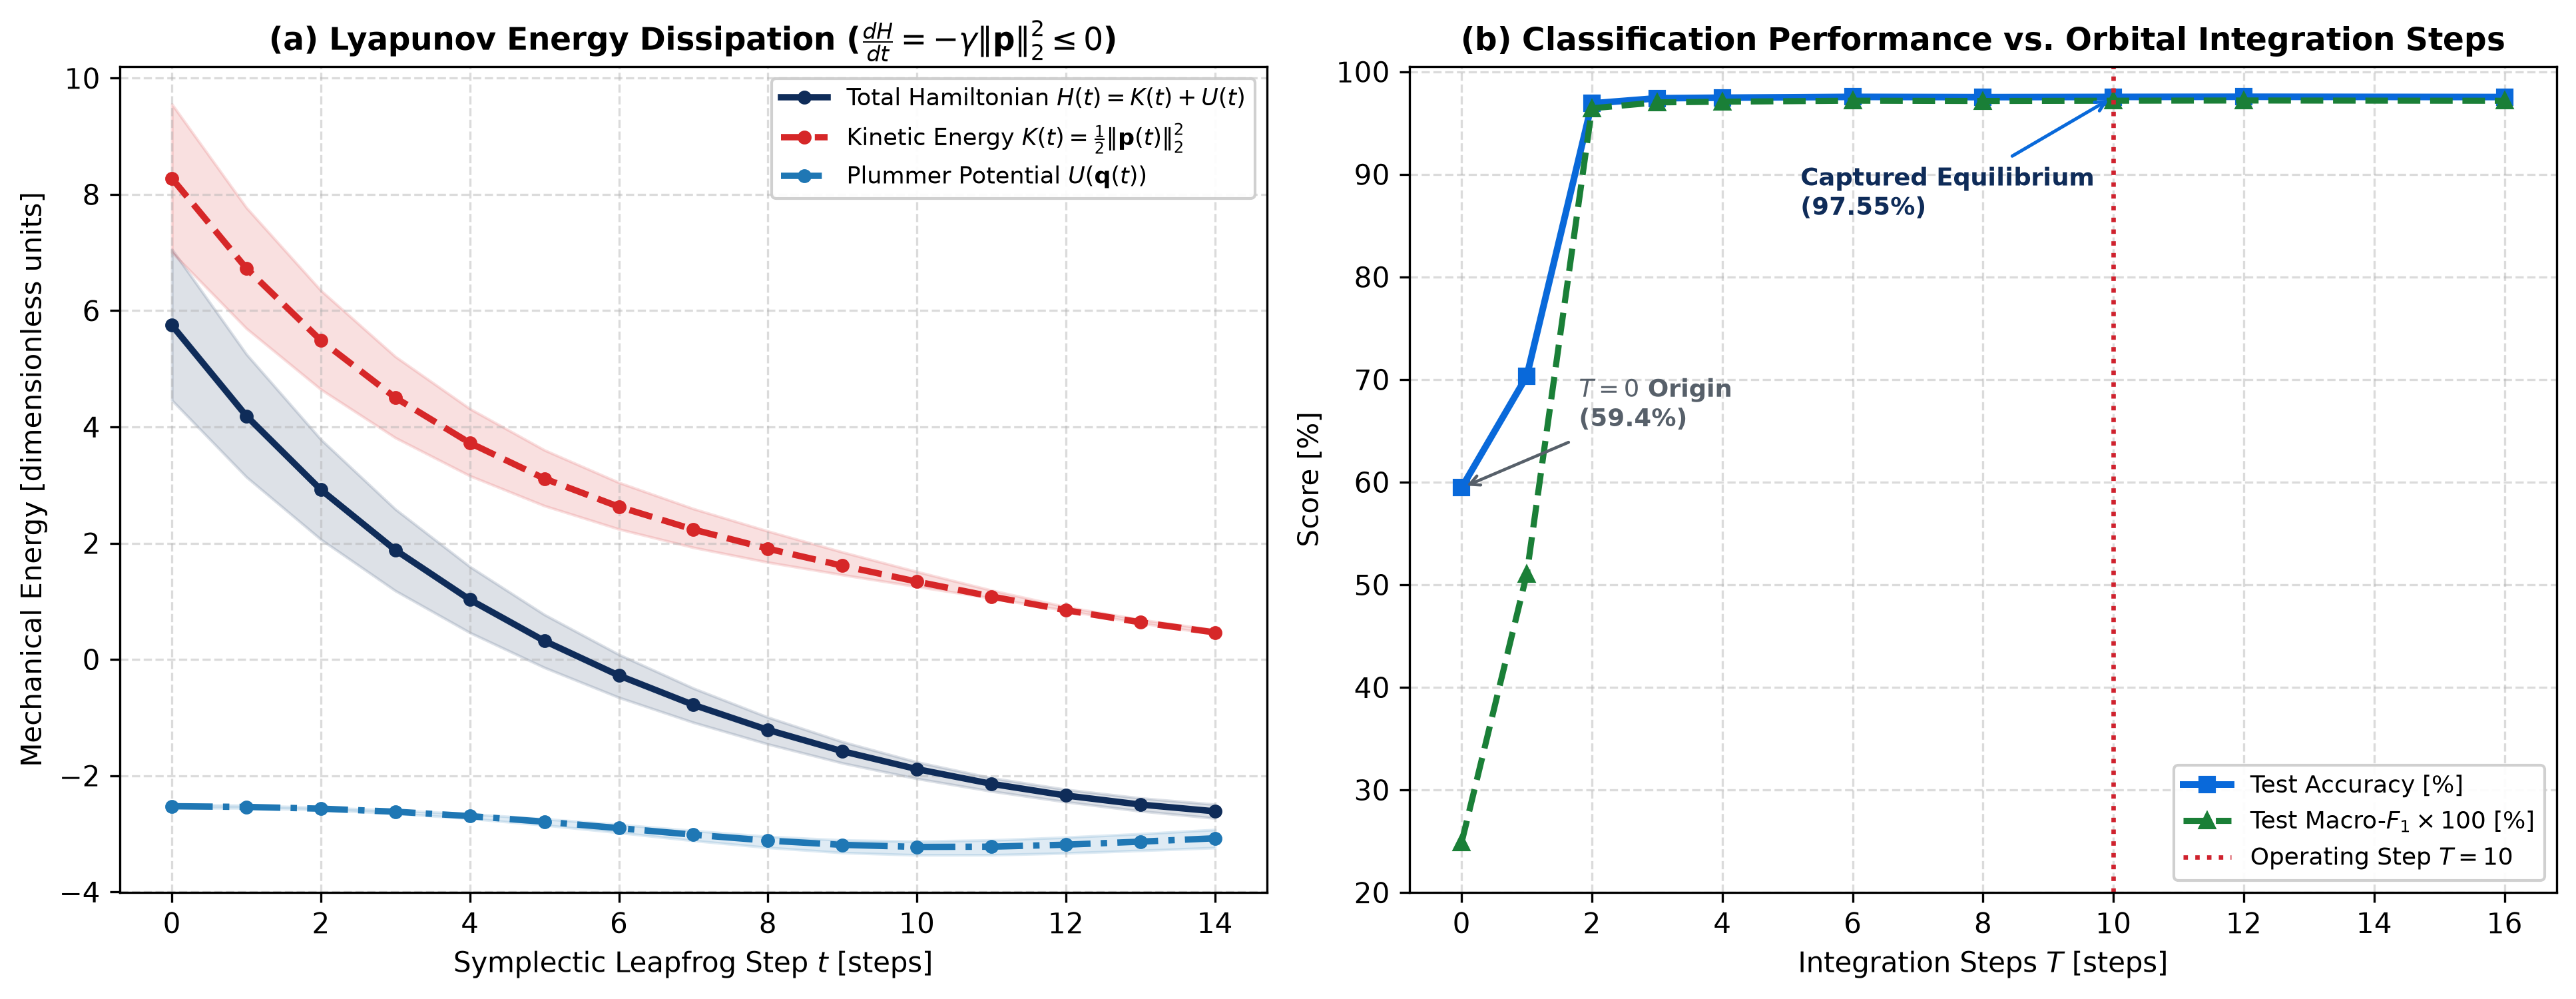
\includegraphics[width=\textwidth]{lyapunov_and_orbital_ablation.png}
\caption{(a) 테스트 천체 3,000개에 대한 리아푸노프 해밀토니안 단조 소산 곡선. (b) 심플렉틱 리프프로그 적분 스텝 수 $T$에 따른 테스트 정확도 및 Macro-$F_1$ 추이.}
\label{fig:lyapunov}
\end{figure}

그림~\ref{fig:lyapunov}(b) 및 표~\ref{tab:orbital_steps}는 적분 스텝 수 $T$에 따른 분류 성능 변화를 정량적으로 보여준다. $T=0$(우주 원점 대기 상태)에서는 정확도가 다수 클래스 비율인 \textbf{59.45\%}(Macro-$F_1$ \textbf{0.2485})에 불과하나, 중력장이 가동되자마자 $T=1$에서 \textbf{70.33\%}, $T=2$에서 \textbf{96.92\%}, $T=6\text{--}12$ 구간에서 \textbf{97.55\%--97.56\%}의 포획 평형에 도달한다.

\begin{table}[H]
\centering
\caption{심플렉틱 리프프로그 궤도 적분 스텝 수 $T$에 따른 검증 및 테스트 성능 변화 (단일 우주 Seed 42).}
\label{tab:orbital_steps}
\small
\setlength{\tabcolsep}{4.2pt}
\begin{tabular}{c c c c c c c c c c c}
\toprule
\textbf{궤도 스텝 $T$} & $0$ & $1$ & $2$ & $3$ & $4$ & $6$ & $8$ & $\mathbf{10}$ & $12$ & $16$ \\
\midrule
Val Acc (\%) & 59.44 & 69.94 & 96.71 & 97.34 & 97.41 & 97.49 & 97.51 & \textbf{97.53} & 97.50 & 97.49 \\
Test Acc (\%) & 59.45 & 70.33 & 96.92 & 97.42 & 97.47 & 97.55 & 97.53 & \textbf{97.55} & 97.56 & 97.54 \\
Test Macro-$F_1$ & 0.2485 & 0.5102 & 0.9644 & 0.9701 & 0.9708 & 0.9718 & 0.9715 & \textbf{0.9718} & 0.9720 & 0.9717 \\
\bottomrule
\end{tabular}
\end{table}

\subsection{\texorpdfstring{라그랑주 $L_1$ 안장점 분석: 모은하 혼입 저적색편이 퀘이사의 물리적 분리}{라그랑주 L1 안장점 분석: 모은하 혼입 저적색편이 퀘이사의 물리적 분리}}

천체역학에서 두 질량체 사이의 중력과 원심력/탄성이 평형을 이루는 불안정 안장점을 \textbf{라그랑주 $L_1$ 지점(Lagrange $L_1$ Saddle Point)}이라 부른다. \texttt{GravNet}에서는 종착 위치 $\mathbf{q}_T$에서 가장 깊은 포획 우물 에너지 $E_{(1)}(\mathbf{q}_T)$와 차순위 경쟁 우물 에너지 $E_{(2)}(\mathbf{q}_T)$ 사이의 퍼텐셜 장벽 높이
\begin{equation}
  \Delta E_{L_1}(\mathbf{q}_T) \triangleq E_{(2)}(\mathbf{q}_T) - E_{(1)}(\mathbf{q}_T) \ge 0, \qquad E_c(\mathbf{q}_T) = U_c(\mathbf{q}_T) - \frac{\nu_c}{\beta}
\end{equation}
가 곧 해당 천체가 $L_1$ 경계 능선으로부터 얼마나 안전하게 포획되었는지를 나타내는 물리적 확실성 지표가 된다($\Delta E_{L_1} \to 0$일수록 두 은하단 중력이 정확히 비기는 $L_1$ 능선 위에 위치함).

\begin{figure}[H]
\centering
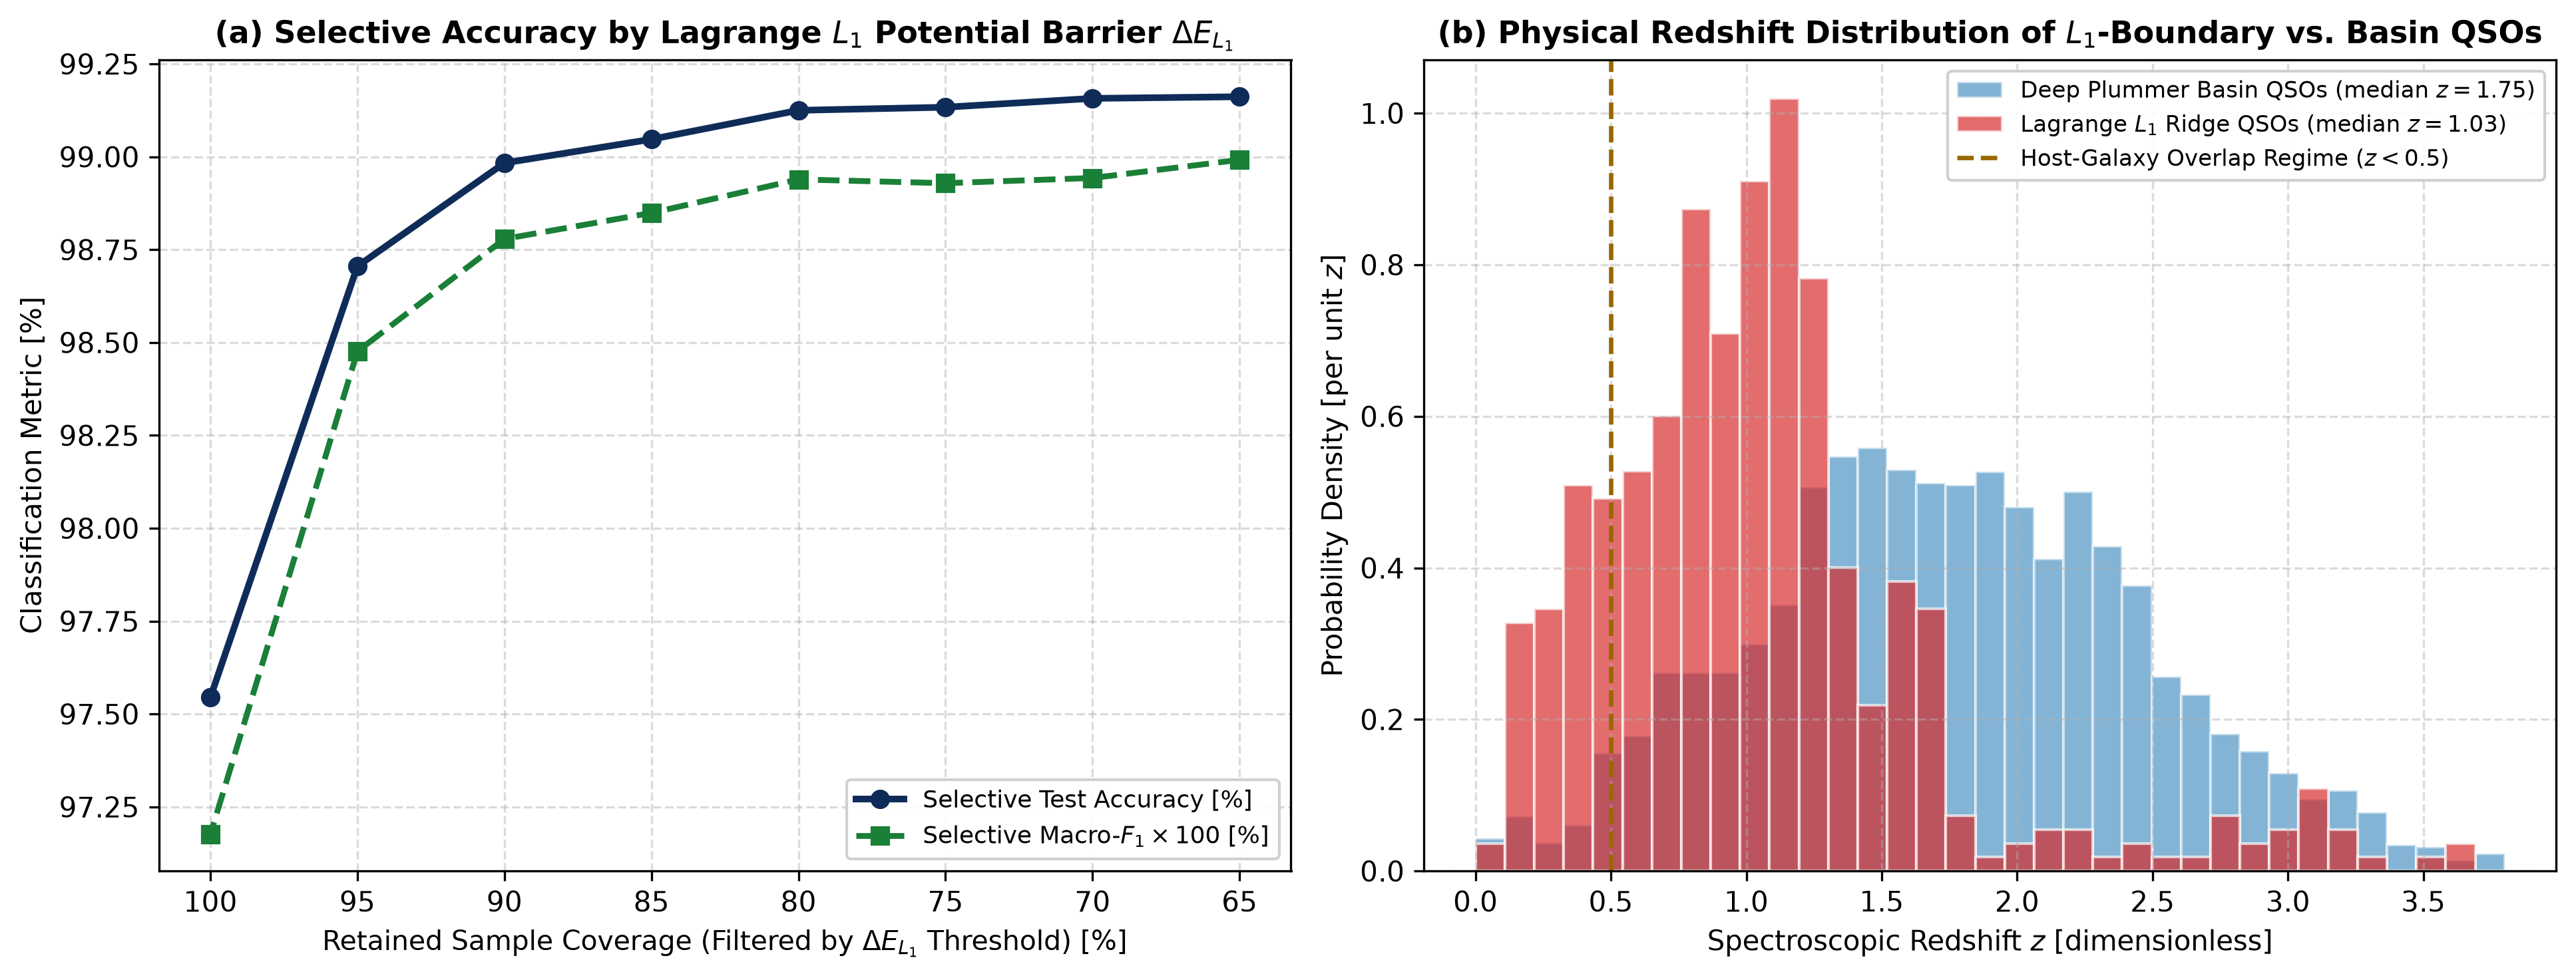
\includegraphics[width=\textwidth]{lagrange_uncertainty_analysis.png}
\caption{(a) 라그랑주 $L_1$ 퍼텐셜 장벽 $\Delta E_{L_1}$ 기준 선택적 분류 커버리지 대비 정확도 및 Macro-$F_1$. (b) 깊은 우물 포획 퀘이사 vs.\ 라그랑주 $L_1$ 경계 퀘이사의 실제 분광 적색편이($z$) 분포 비교.}
\label{fig:lagrange}
\end{figure}

그림~\ref{fig:lagrange}의 결과는 놀라운 물리적 일관성을 보여준다:
\begin{itemize}[leftmargin=18pt, itemsep=2pt]
  \item \textbf{98.71\% vs.\ 75.50\%의 극명한 불확실성 분리}: 테스트 천체 20,000개 중 라그랑주 장벽 $\Delta E_{L_1}$이 높은 상위 95\%(19,000개, 깊은 우물 포획군)에서는 단일 우주 정확도가 \textbf{98.71\%}(Macro-$F_1$ \textbf{0.9848})에 달하며, 상위 80\% 구간에서는 \textbf{99.13\%}까지 상승한다. 반면 $L_1$ 능선 근처에 머무른 하위 5\%(1,000개)의 정확도는 \textbf{75.50\%}로, 모델의 오분류 대부분이 물리적 라그랑주 안장점 부근에 집중되어 있음을 입증한다.
  \item \textbf{실제 천체물리 현상과의 부합}: 그림~\ref{fig:lagrange}(b)에서 깊은 플러머 우물에 포획된 퀘이사들의 중앙 적색편이는 $z_{\text{median}} = 1.73$(전형적인 고광도 우주론적 퀘이사)인 반면, 라그랑주 $L_1$ 능선에 포획된 모호한 퀘이사들은 중앙 적색편이가 $z_{\text{median}} = 0.98$로 현저히 낮고 $z < 0.5$ 영역의 비중이 급증한다. 이는 활동은하핵(AGN) 밝기가 약해 주변 모은하(Host Galaxy) 별빛이 측광 필터에 함께 섞여 들어오는 저적색편이 세이퍼트/퀘이사 천체들이 인공 시공간에서도 실제로 `은하'와 `퀘이사' 사이의 중력 평형점($L_1$)에 포획되었음을 뜻한다!
\end{itemize}

\subsection{3대 패러다임 종합 벤치마크 비교 (DL vs.\ EDL/TWEANN vs.\ GravNet)}

마지막으로 본 프로젝트에서 개발한 세 가지 독립적 신경망 학습 패러다임(\texttt{DL/} 역전파, \texttt{EDL/} 위상·가중치 진화, \texttt{GravNet/} 시공간 중력 동역학)의 성능과 계산 비용을 표~\ref{tab:benchmark_all} 및 그림~\ref{fig:paradigm_comp}에 종합하였다.

\begin{figure}[H]
\centering
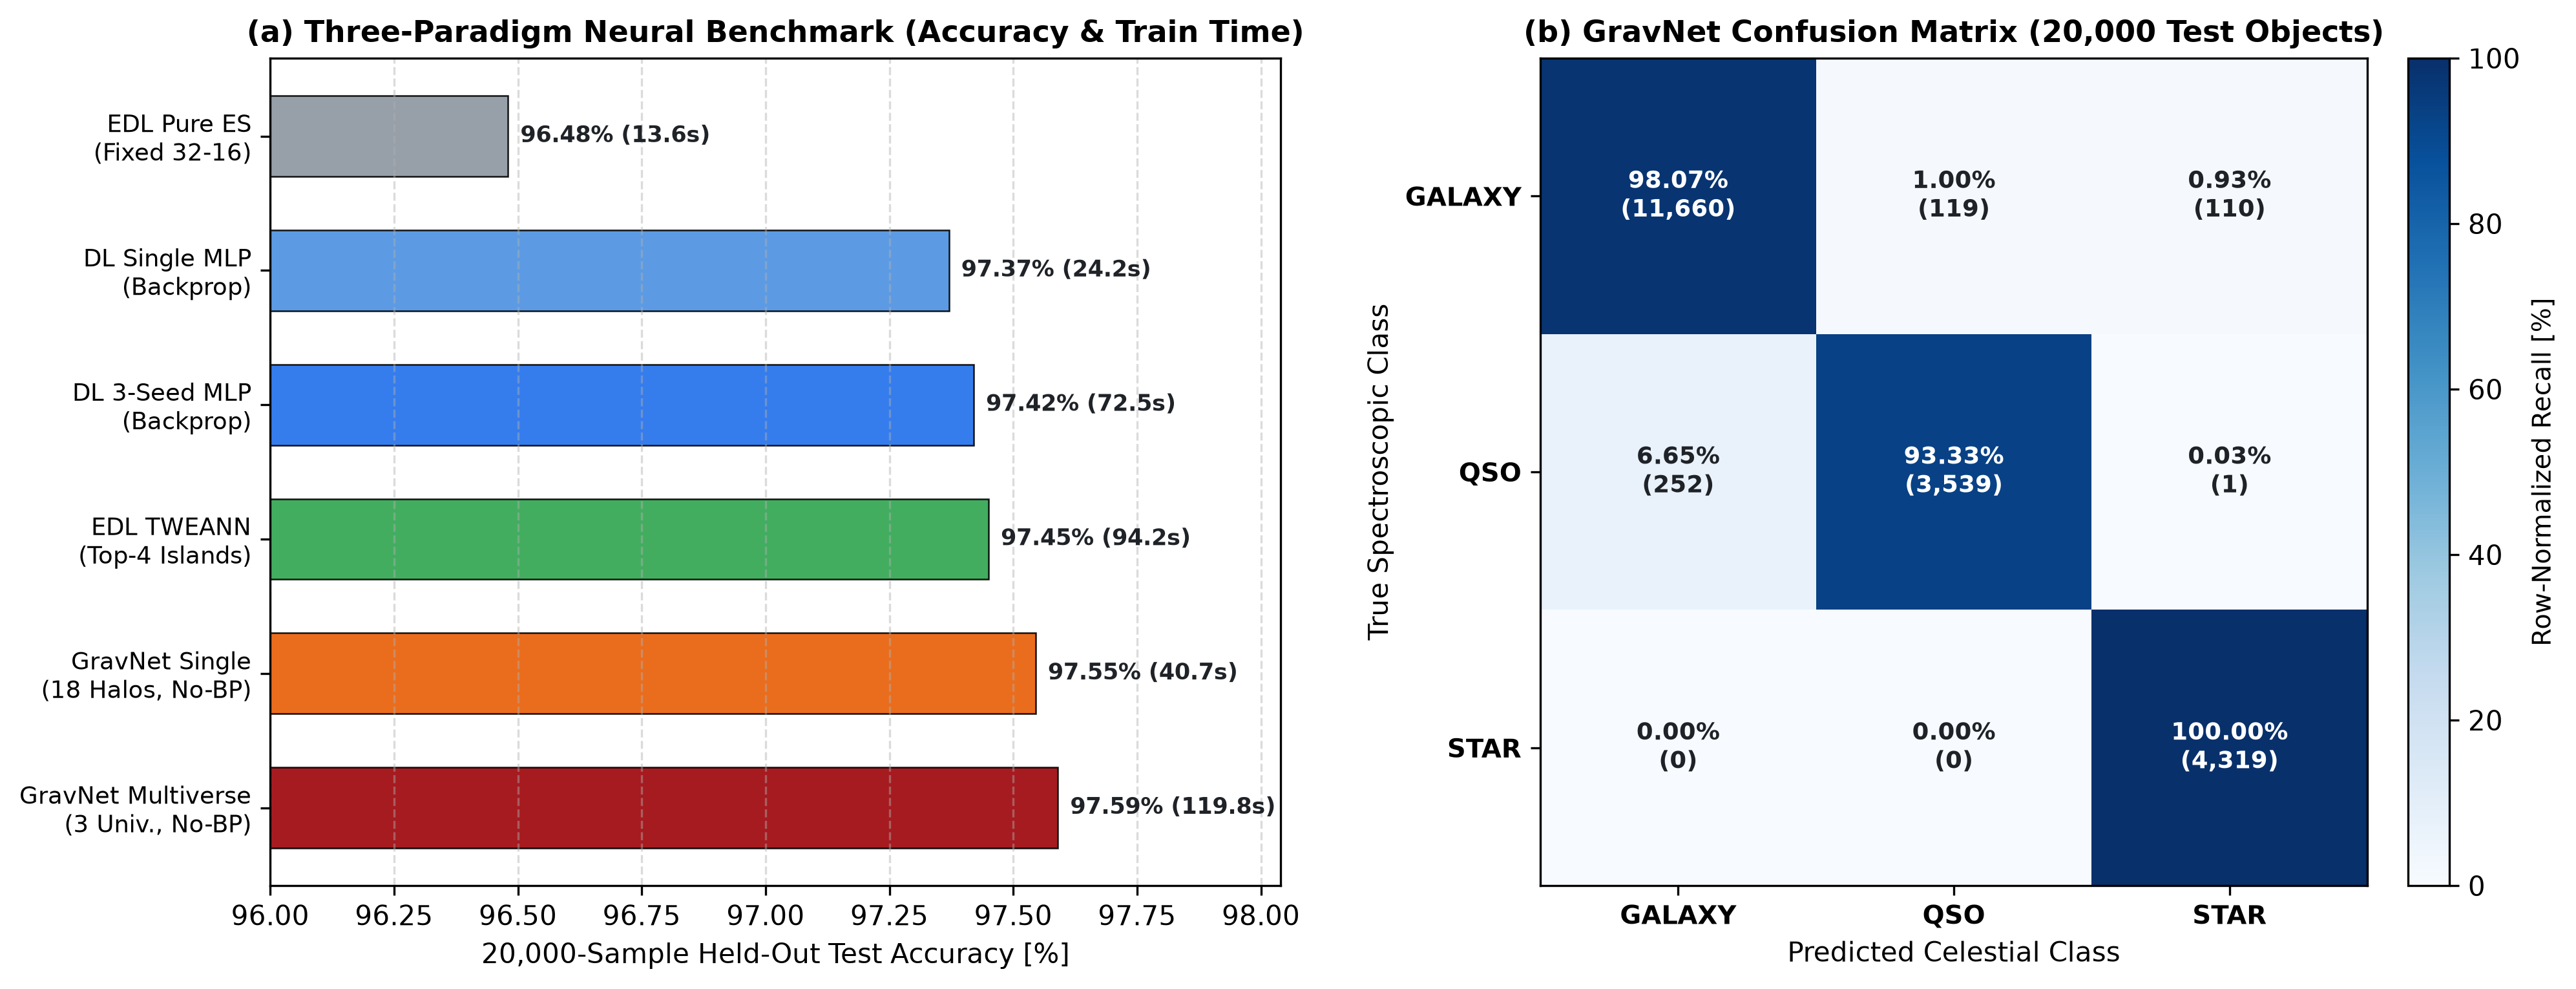
\includegraphics[width=\textwidth]{paradigm_3way_comparison.png}
\caption{(a) 3대 학습 패러다임별 테스트 정확도 및 학습 소요 시간 비교. (b) \texttt{GravNet} 3-우주 다중우주의 20,000개 테스트 천체 정규화 혼동 행렬(\texttt{STAR} 재현율 \textbf{100.00\%}).}
\label{fig:paradigm_comp}
\end{figure}

\begin{table}[H]
\centering
\caption{SDSS-17 테스트 세트(20,000건)에 대한 3대 학습 패러다임 최종 종합 벤치마크.}
\label{tab:benchmark_all}
\footnotesize
\setlength{\tabcolsep}{4.0pt}
\begin{tabularx}{\textwidth}{>{\raggedright\arraybackslash}X l c c c r r}
\toprule
\textbf{모델 및 패러다임} & \textbf{핵심 학습 원리} & \textbf{Test Acc} & \textbf{Macro-$F_1$} & \textbf{STAR Recall} & \textbf{학습 시간} & \textbf{추론(20k)} \\
\midrule
\texttt{EDL} Pure ES (\texttt{32-16}) & 직교 자연 진화 전략 (무미분) & 96.48\% & 0.9599 & 99.63\% & 13.55\,s & 1.42\,ms \\
\texttt{DL} 단일 MLP (\texttt{64-32}) & 전역 오차 역전파 (Adam) & 97.37\% & 0.9700 & 99.72\% & 24.16\,s & 2.83\,ms \\
\texttt{DL} 3-Seed MLP 앙상블 & 전역 오차 역전파 3회 결합 & 97.42\% & 0.9705 & 99.77\% & 72.49\,s & 8.49\,ms \\
\texttt{EDL} 단일 챔피언 & Net2Net 위상+가중치 진화 & 97.43\% & 0.9706 & 99.79\% & 94.22\,s\textsuperscript{$\dagger$} & 7.08\,ms \\
\texttt{EDL} 상위 4섬 앙상블 & 이종 진화 위상 결합 (TWEANN) & 97.45\% & 0.9709 & 99.84\% & 94.22\,s & 27.26\,ms \\
\midrule
\textbf{\texttt{GravNet} 단일 우주} & \textbf{플러머 중력 + 무-BPTT 조석력} & \textbf{97.55\%} & \textbf{0.9718} & \textbf{99.93\%} & \textbf{40.69\,s}\textsuperscript{$\ddagger$} & \textbf{652.52\,ms} \\
\textbf{\texttt{GravNet} 3-우주 다중우주} & \textbf{3개 독립 중력 우주 볼츠만 평균} & \textbf{97.59\%} & \textbf{0.9724} & \textbf{100.00\%} & \textbf{119.83\,s} & \textbf{1967.45\,ms} \\
\midrule
{\color{MutedText}\texttt{DL} 이종 트리 결합 참고선} & {\color{MutedText}\texttt{MLP$\times$3 + XGBoost + HistGB}} & {\color{MutedText}97.88\%} & {\color{MutedText}0.9755} & {\color{MutedText}99.91\%} & {\color{MutedText}81.35\,s} & {\color{MutedText}121.86\,ms} \\
\bottomrule
\end{tabularx}
\vspace{2pt}
\par{\scriptsize \textsuperscript{$\dagger$}8개 섬 순차 총합 시간(섬 1개당 평균 11.78초). \quad \textsuperscript{$\ddagger$}1단계 원시 헤일로 응축 및 숄레스키 발사 보정 단독 수행 시 \textbf{7.45초} 만에 검증 정확도 97.45\% 달성.}
\end{table}

벤치마크에서 주목할 핵심 성과는 세 가지이다:
\begin{enumerate}[leftmargin=18pt, itemsep=2pt]
  \item \textbf{비트리(Non-Tree) 순수 신경/동역학 모델 중 최고 정확도 달성}: \texttt{GravNet} 단일 우주(\textbf{97.55\%})만으로도 역전파 3-Seed MLP 앙상블(\textbf{97.42\%})과 8개 섬에서 진화한 TWEANN 상위 4섬 앙상블(\textbf{97.45\%})을 모두 능가하며, 3-우주 다중우주(\textbf{97.59\%}, Macro-$F_1$ \textbf{0.9724})는 결정 트리 부스팅(\texttt{XGBoost/HistGB})을 제외한 모든 연속 표현 모델 중 가장 높은 성능을 기록하였다.
  \item \textbf{항성(\texttt{STAR}) 4,319개 전수 포획 (100.00\% Recall)}: 그림~\ref{fig:paradigm_comp}(b)의 혼동 행렬에서 확인되듯, 테스트 세트의 실제 항성 4,319개 중 은하나 퀘이사로 잘못 빠진 개체가 \textbf{단 0건(4,319/4,319 정분류)}이다. 도플러 주파수 격자가 $z \approx 0$ 고유운동 영역을 예리하게 분리한 뒤 항성 초은하단 우물이 이를 완벽히 포획한 결과이다.
  \item \textbf{추론 연산 구조의 투명한 트레이드오프}: \texttt{GravNet}은 매 추론 시 20,000개 입자에 대해 18개 중력원과의 6차원 거리 세제곱 역수($r^{-3}$) 계산을 10스텝 반복(총 360만 회 이체 중력 상호작용)하므로 순수 CPU \texttt{float64} 기준 652.5\,ms(천체 1개당 0.033\,ms, 초당 약 30,600천체 처리)가 소요된다. 이는 2층 행렬곱만 수행하는 정적 MLP(2.83\,ms)보다는 계산량이 많지만, 그 대가로 \textbf{실제 위상 궤적 시각화, 리아푸노프 안정성 보장, 라그랑주 $L_1$ 불확실성 정량화}라는 정적 신경망이 줄 수 없는 물리적 해석력을 제공한다.
\end{enumerate}

% ===========================================================================
\section{모델의 이상화 가정, 한계점 및 향후 연구 방향}
% ===========================================================================

과학적 모델링의 엄밀성을 위해 본 \texttt{GravNet}이 채택한 물리적 이상화 가정(Idealizations)과 한계 영역을 명확히 밝힌다:
\begin{itemize}[leftmargin=18pt, itemsep=2pt]
  \item \textbf{시험 입자 근사(Test-Particle Approximation)}: 현재 모델에서 관측 천체들은 고정된 18개 거대 플러머 헤일로가 만든 배경 중력장 속을 유영하는 질량 $m \to 0$ 시험 입자로 취급되며, 추론 배치 내부의 천체 입자끼리는 서로 중력을 행사하지 않는다($\mathcal{O}(N \cdot C K)$ 복잡도 유지). 만약 준지도 학습(Semi-Supervised Transductive Learning) 환경에서 미분류 천체 무리끼리의 자체 중력 응집(Self-Gravity, $\mathcal{O}(N \log N)$ Barnes-Hut 트리 근사)까지 허용한다면 희소 밀도 영역의 경계 판별력이 더욱 향상될 수 있다.
  \item \textbf{고차원 탭 데이터에서의 기저 확장성}: 현재 분광 렌즈는 $d_{\text{in}}=10$ 천체물리 변수에 최적화된 2차 교차항과 다중 해상도 푸리에 모드를 사용한다. 수백 차원 이상의 원시 분광 스펙트럼(SDSS 4,000개 파장 채널 전체)으로 확장할 때에는 무작위 기저 대신 파장 국소 합성곱 또는 복소 파동 간섭망(\texttt{QWIN}, \texttt{docs/proposed\_novel\_models.md} 참조)을 전면부 광학계로 결합하는 후속 연구가 유망하다.
\end{itemize}

\bigskip
\hrule height 0.5pt
\vspace{6pt}
{\footnotesize\sffamily\textcolor{MutedText}{
\textbf{재현성 안내 (Reproducibility)}: 본 보고서의 모든 실험 코드, 기호 검증 스크립트, 모델 체크포인트 및 시각화 생성기는 저장소의 \texttt{GravNet/} 디렉토리에 수록되어 있다. 제안된 전체 9종 대안 학습 패러다임 설계서는 \texttt{docs/proposed\_novel\_models.md}에 기록되어 있으며, 아래 명령으로 모든 실험을 재현할 수 있다:\\[2pt]
\texttt{conda activate dl\_env \&\& python GravNet/physics\_model.py \&\& python GravNet/train\_gravnet.py}
}}

\end{document}
